\section{Manual de usuario}\label{Manual usuario}

Para el correcto uso de la aplicación, el conjunto de acciones que se pueden realizar en dicho programa serán definidas a continuación. También, la distribución de las secciones de la interfaz junto a su explicación y funcionalidad.\bigskip

Cuando se ejecute el programa por primera vez en la pantalla se debe mostrar la siguiente interfaz de usuario:

\begin{figure}[!h]
    \centering
    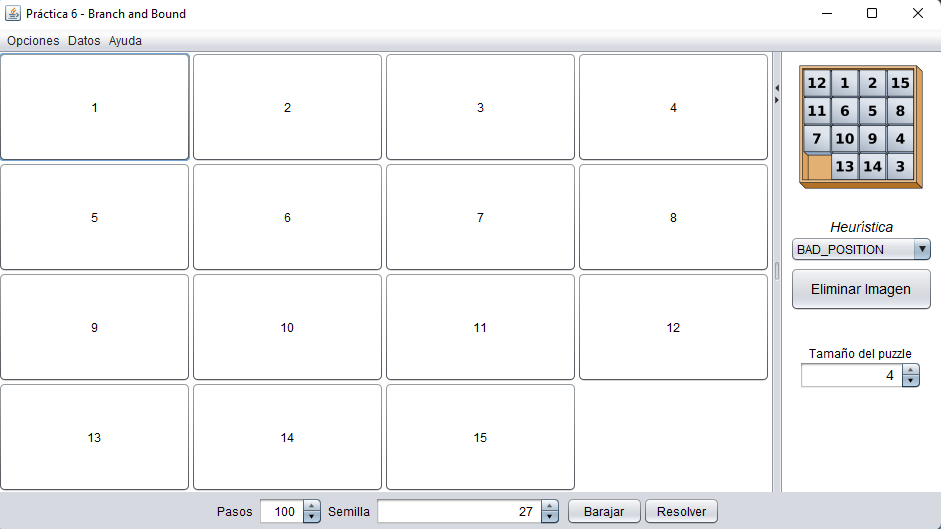
\includegraphics[width=\linewidth]{Usage/img/GUI.png}
    \caption{Interfaz de usuario.}
    \label{fig:User_interface}
\end{figure}

\subsection{Menu}\label{Manual usuario, Header}

El menú de la aplicación consiste en la barra que se sitúa debajo del marco superior de la ventana. En esta se puede encontrar un conjunto de opciones para que el usuario pueda interactuar con la aplicación, modificar y analizar el comportamiento de esta. En concreto, se encuentran las opciones de \say{Opciones}, \say{Datos} y \say{Ayuda}, respectivamente.\bigskip

En la primera se sitúan las acciones para salir del programa y para iniciar las ventanas de estadísticas explicadas anteriormente en los apartados \ref{Stats JVM} y \ref{Stats Algt}.\bigskip

En la segunda opción llamada \say{Datos} encontramos en primer lugar, la opción para crear una base de datos y cargar los datos. Por otra parte, tenemos la opción de cargar una imagen directamente.\bigskip

En la tercera opción se encuentra un menú desplegable con un manual de usuario con la explicación del funcionamiento de la aplicación.
 
\subsection{Main}

El \say{Main} es el bloque principal de la vista, donde se representará el problema del Puzzle 15. El usuario no podrá interactuar directamente con las casillas para moverlas, sino que, tendrá diferentes opciones para poder resolver el problema. Entre las opciones se encuentran: la heurística, el tamaño del puzzle, los pasos para resolverlo, la semilla, un botón para mezclar las casillas y por último, otro botón para resolver el problema.

\subsection{Sidebar}\label{Sidebar}

El \say{Sidebar} contiene un conjunto de opciones para modificar los datos y el modo de ejecución de la aplicación. A continuación, se explicará cada una de estas opciones y su función.\bigskip

En primer lugar, se encuentra la opción para seleccionar la \say{Heurística}. En esta, se puede escoger el método de resolución del algoritmo a aplicar sobre el problema. Se han definido las siguientes heurísticas:

\begin{itemize}
    \item BAD POSITION
    \item MANHATTAN
    \item LINEAR CONFLICT
\end{itemize}
\bigskip

Debajo de este, se encuentra un botón para eliminar la imagen actual y volver a la primera pantalla. \bigskip

En tercer lugar se encuentra la opción para seleccionar el tamaño del puzzle, el tamaño mínimo será de 2x2 y el tamaño máximo de 50x50.

\subsection{Footer}\label{Footer}

En la sección \say{Footer}, se hallan varias opciones para interactuar con la interfaz y también con el algoritmo a ejecutar. \bigskip

En primer lugar tenemos una opción para seleccionar el número de veces que se va a realizar el proceso de barajado.\bigskip

En segundo lugar la semilla de aleatoriedad para generar el número aleatorio. \bigskip

En tercer lugar, encontramos el botón \say{Barajar}, este botón realiza la mezcla de las casillas, cambiando las posiciones de unas por otras. Se puede clicar las veces que el usuario desee.\bigskip

Por último, el botón \say{Resolver} que ejecutará el algoritmo con los parámetros que le hayamos indicado en la UI.

\subsection{Ejemplo ejecución}

Al iniciar la aplicación se mostrará una interfaz como la expuesta en la imagen \ref{fig:User_interface}. Para poder iniciar la ejecución del algoritmo, el usuario tendrá que mezclar las casillas, y pulsar el botón de resolver. Además, tiene la opción de cambiar los pasos o la semilla de aleatoriedad. Por otra parte, el usuario podrá seleccionar la heurística para la resolución del problema y añadir imágenes para hacerlo visual. A continuación, la siguiente imagen, muestra un ejemplo de la interfaz tras la ejecución:

\begin{figure}[!h]
    \centering
    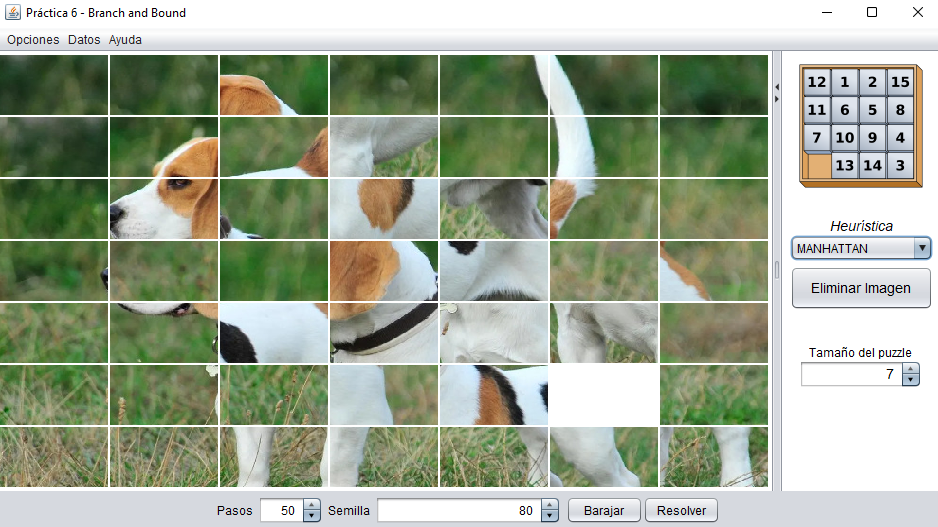
\includegraphics[width=\linewidth]{Usage/img/ejecucion.png}
    \caption{Interfaz de usuario en ejecución.}
    \label{fig:Ejemplo ejecución}
\end{figure}

Tras ejecutar el algoritmo, se mostrará al usuario paso por paso como se resuelve el mismo.  \bigskip

A partir de aquí, el usuario puede salir del programa con el botón del menú, cargar una base de datos, cargar una imagen, cambiar la heurística, el tamaño del puzzle o las imágenes y ver estadísticas de la ejecución, ver apartados \ref{Stats JVM} y \ref{Stats Algt}.
